\documentclass[twoside]{article}
\usepackage{../quiz}
\usepackage{fancyhdr}

\pagestyle{fancy}
\renewcommand{\headrulewidth}{0pt}
\cfoot{}
\rfoot{Solutions at \textbf{\href{http://owenjow.xyz/cs61a/section-quizzes/}{owenjow.xyz/cs61a/section-quizzes}}. Credit to Brian Hou for the questions.}
\renewcommand{\footrulewidth}{0.4pt}

\lstset{
    language=Python,
    basicstyle=\ttfamily,
    showstringspaces=false
    keywordstyle=\color{black},
    commentstyle=\color{black},
    stringstyle=\color{black},
    escapeinside={<*}{*>},
    moredelim=**[is][\color{red}]{@}{@},
}

\def\semester{Spring 2017}
\newcommand{\solution}[1]{{\color{red}#1}}

%%% Actual, flexible content begins here %%%
\title{\sc Quiz 5 \solution{Solutions}}

\begin{document}
\maketitle

\begin{enumerate}
%%% Q1 %%%
\q{5}{LoopList}

Implement a class \lstinline{LoopList} that has a method \lstinline{at_index}. If \lstinline{at_index} is called with an index that is too large, the \lstinline{LoopList} will loop around back to the beginning.
\vspace{0.1in}

\begin{lstlisting}
class LoopList:
    """
    >>> x = LoopList([3, 1, 4])
    >>> [x.at_index(i) for i in range(10)]  # loops around!
    [3, 1, 4, 3, 1, 4, 3, 1, 4, 3]
    """
    @def __init__(self, lst):
        self.lst = lst
    
    def at_index(self, i):
        return self.lst[i % len(self.lst)]@
\end{lstlisting}

\newpage

%%% Q2 %%%
\q{5}{Berkeley Landmark \#158}

Draw the environment diagram. (This is very hard!)
\vspace{0.1in}

\begin{lstlisting}
def campa(nile):
    def ding(ding):
        nonlocal nile
        def nile(ring):
            return ding
    return nile(ding(1914)) + nile(1917)

ring = campa(lambda nile: 100)
\end{lstlisting}

\begin{figure}[ht!]
\hspace*{5mm}
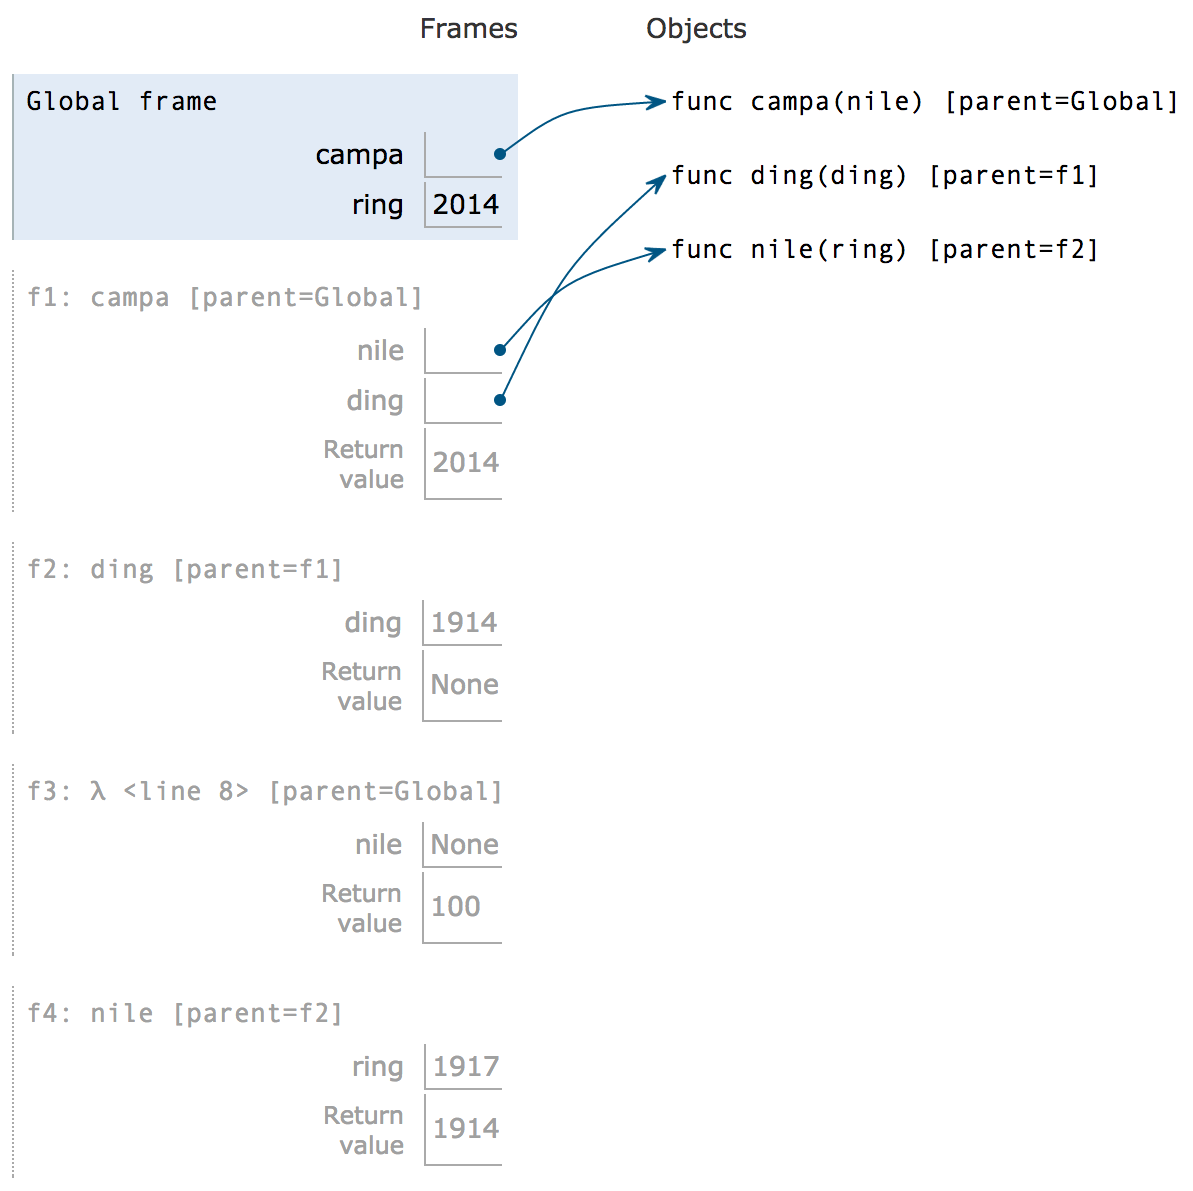
\includegraphics[width=155mm]{../../../../images/quiz5_sol.png}
\end{figure}

\end{enumerate}
\end{document}
